\documentclass[a4paper]{article}

\usepackage{fullpage} % Package to use full page
\usepackage{parskip} % Package to tweak paragraph skipping
\usepackage{tikz} % Package for drawing
\usepackage{amsmath}
\usepackage{hyperref}
\usepackage{ctex}
\usepackage{amssymb}
\usepackage{amsthm}
\usepackage{indentfirst}
\setlength{\parindent}{2em}
\usepackage{array}
\usepackage{graphicx}
\usepackage{float} 
\usepackage{subfigure}

\renewcommand\thefigure{\thesection.\arabic{figure}}
\makeatletter
\@addtoreset{figure}{section}
\makeatother

\renewcommand\thesubfigure{\thesection.\arabic{figure}(\alph{subfigure})}
\makeatletter
\@addtoreset{figure}{section}
\makeatother

\makeatletter
\renewcommand \theequation {%
	\ifnum \c@section>\z@ \@arabic\c@section.\fi \ifnum \c@subsection>\z@
	\@arabic\c@subsection.\fi\ifnum \c@subsubsection>\z@
	\@arabic\c@subsubsection.\fi\@arabic\c@equation}
\@addtoreset{equation}{section}
\@addtoreset{equation}{subsection}
%\setcounter{section}{-1}
\makeatother
\newtheorem{theorem}{\hspace{2em}定理}[section]
\hypersetup{
	colorlinks=true,
	linkcolor=black
}

\title{高等数值分析}
\author{罗雁天 \\
2018310742}
\date{\today}

\begin{document}

%\maketitle
\newcommand{\HRule}{\rule{\linewidth}{0.5mm}}
\begin{titlepage}
	\begin{center}
		% Upper part of the page
		
\includegraphics[width=0.4\textwidth]{Tsinghua2.png}\\[1cm]
		\textsc{\Large \texttt{高等数值分析}}\\[1cm]
		% Title
		\HRule \\[1cm]
		{\Huge \bfseries 病态线性方程组的求解}\\[0.4cm]
		\HRule \\[3.5cm]
		% Author and supervisor
		\begin{minipage}{0.4\textwidth}
			\begin{center}
				\Large
				\begin{tabular}{cc}
					\texttt{作者:} & 罗雁天 \\[0.5cm]
					\texttt{学号:} & 2018310742 \\[0.5cm]
					\texttt{日期:} & \today
				\end{tabular}
			\end{center}
		\end{minipage}
		\vfill
	\end{center}
\end{titlepage}

\tableofcontents
\newpage

\section{题目描述}
理论分析表明,数值求解病态线性方程组很困难。考虑求解如下的线性方程组,$Hx=b$,其中$H$是Hilbert矩阵,$H=(h_{ij}),h_{ij}=\frac{1}{i+j-1},i,j=1,2,\cdots,n$。本次大作业从条件数、高斯消去法、Jacobi迭代法、Gauss-Seidel迭代法、SOR迭代法等角度分析上述病态线性方程组并进行对比。

\section{Hilbert矩阵2-条件数和阶数的关系}
\subsection{使用Matlab自带的cond()函数进行计算}
由于Matlab自带了求2-条件数的函数$cond()$,因此我们首先采用此种方式讨论Hilbert矩阵2-条件数和阶数的关系。

我们首先计算了几个低阶的条件数如表\ref{tab:table1}所示。从表中我们可以看出,随着矩阵阶数$n$的增长,2-条件数增加幅度很快,因此我们采用对数坐标绘制2-条件数和矩阵阶数n的关系曲线。

\begin{table}[htbp]
	\centering
	\caption{Hilbert矩阵2-条件数与阶数的关系表格}
	\label{tab:table1}
	\begin{tabular}{|c|c|c|c|c|c|}
		\hline
		阶数n & 1 & 2 & 3 & 4 & 5 \\
		\hline
		2-条件数 & 1.0000 & 19.2815 & 524.0568 & 15513.7387 & 476607.2502\\
		\hline
	\end{tabular}
\end{table}

取矩阵的阶数从$1\to100$,在对数坐标下绘制2-条件数和矩阵阶数n的关系曲线如图\ref{fig:1}所示。从图中我们可以看出,当阶数较低(大约$1\to 13$)时,对数化2-条件数大约与阶数呈现线性关系,当阶数变高时,对数化的2-条件数波动起来,不再增加,根据我们对Hilbert矩阵病态性的知识,图\ref{fig:1}中阶数较大时的曲线显然不正确,由此可以说明Matlab自带的cond()函数在矩阵阶数较高时计算的条件数误差较大。因此我们考虑另一种方法计算矩阵的条件数。

\begin{figure}[!h]
	\centering
	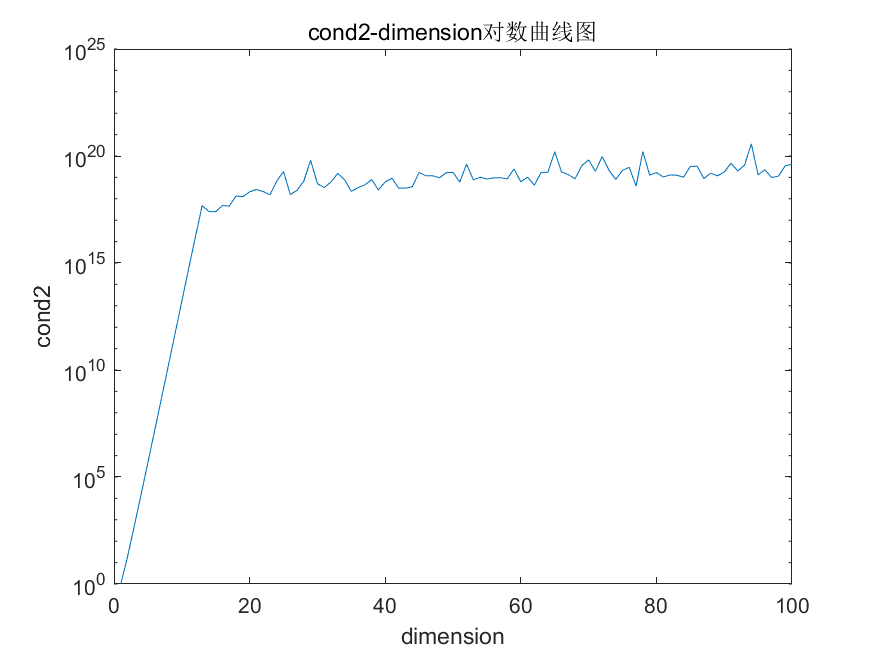
\includegraphics[width=0.8\textwidth]{../code/result/logcond2}
	\caption{\label{fig:1}使用cond()函数计算的2-条件数和矩阵阶数n在对数坐标下的曲线}
\end{figure}

\subsection{使用2-条件数的定义进行计算}
根据2-条件数的定义$cond_2(H)=||H||_2||H^{-1}||_2$,Matlab中有专门针对Hilbert矩阵逆矩阵的函数$invhilb()$,因此我们可以采用定义法来计算Hilbert矩阵的2-条件数。同样在对数坐标下,绘制出此种方法计算出的2-条件数和矩阵阶数的关系图如图\ref{fig:2}所示,从此图中可以看出,随着矩阵阶数的增加,对数化的2-条件数近似与阶数呈现线性关系,符合我们对Hilbert矩阵病态性的理解。

我们将对数化的2-条件数和矩阵阶数进行线性回归,得到拟合公式为: $cond2=10^{1.5257n-2.0758}$,相关系数$r\approx 1$,拟合之后图像如图\ref{fig:3}所示。

\begin{figure}[!h]
	\centering
	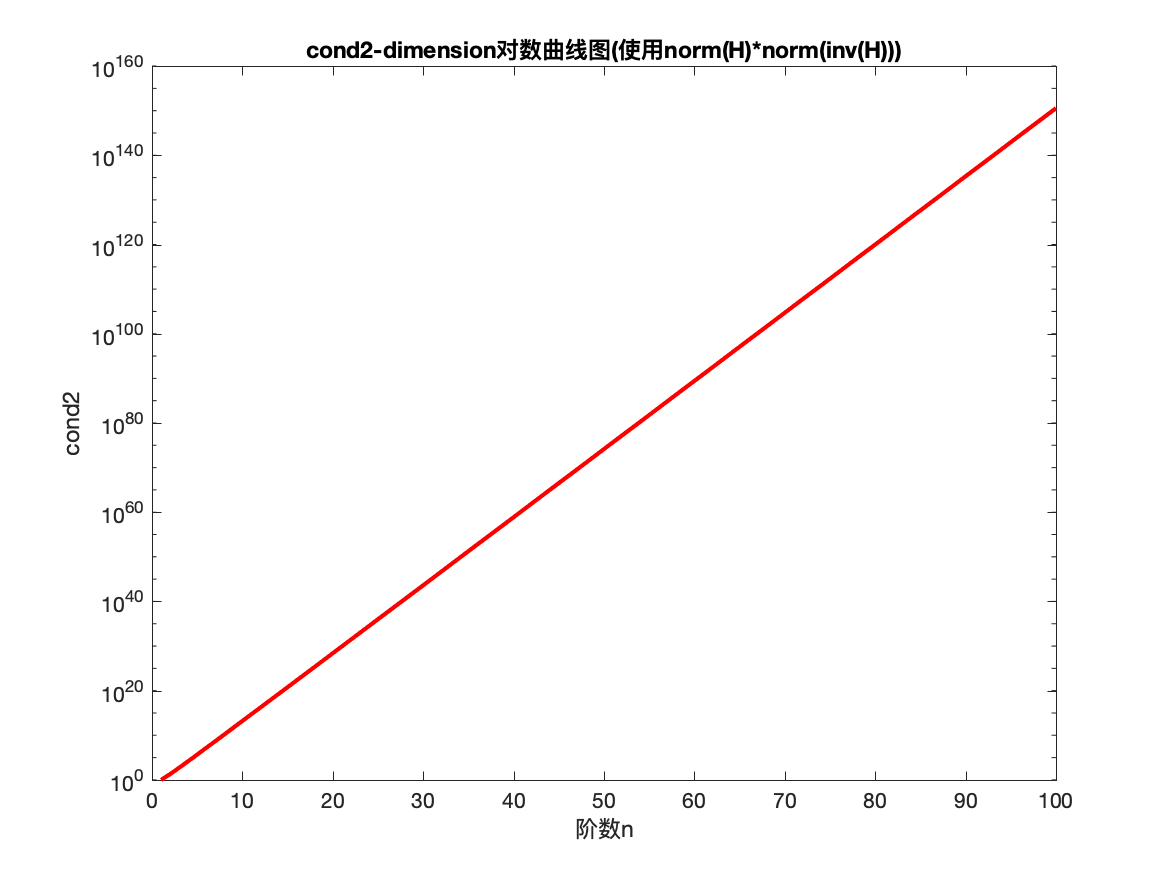
\includegraphics[width=0.8\textwidth]{../code/result/alogcond2}
	\caption{\label{fig:2}使用定义计算的2-条件数和矩阵阶数n在对数坐标下的曲线}
\end{figure}

\begin{figure}[!h]
	\centering
	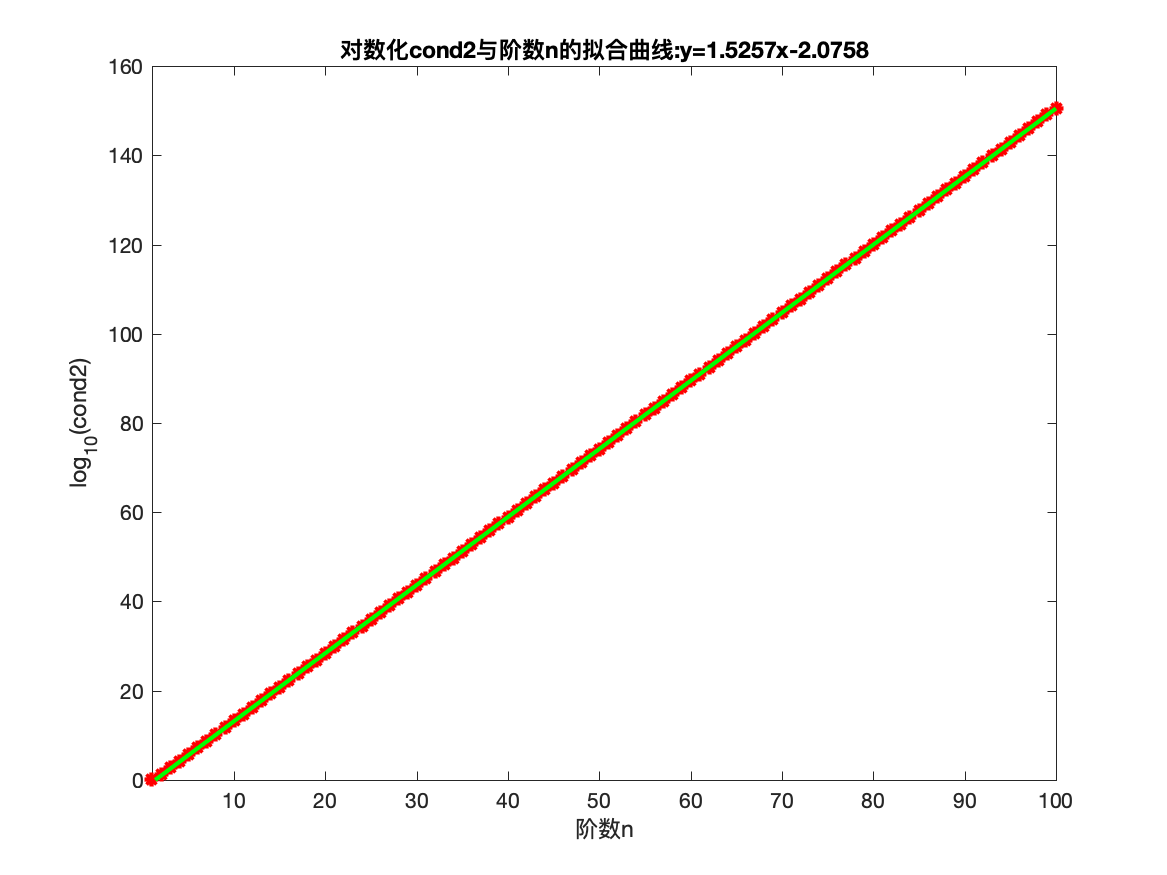
\includegraphics[width=0.8\textwidth]{../code/result/cond2fit}
	\caption{\label{fig:3}使用定义计算的2-条件数和矩阵阶数n在对数坐标下的曲线}
\end{figure}

\section{Gauss消去法}
用Gauss消去法将Hilbert矩阵消成上三角矩阵,然后求解结果。我们将阶数$n=2,5,10,20,50,100$的误差列表如表\ref{tab:table2}所示,从表中我们可以看出,随着矩阵阶数的增加,Gauss消去法的误差上升较快,当阶数为13时,误差就已经达到了3.0655,相对误差已经很大了,因此Gauss消去法不适和高阶Hilbert矩阵求解。我们绘制出$n=1\to100$时的Gauss消去法求解的相对误差曲线如图\ref{fig:4}所示。

\begin{table}[htbp]
	\centering
	\caption{Gauss消去法相对误差与阶数关系表格}
	\label{tab:table2}
	\begin{tabular}{|p{4cm}<{\centering}|p{6cm}<{\centering}|}
		\hline
		阶数n & Gauss消去法的相对误差 \\
		\hline
		2 & 5.66104886700368e-16 \\
		\hline
		5 & 1.55303820484067e-12 \\
		\hline
		10 & 0.000223773106799740 \\
		\hline
		20 & 23.5417423737487 \\
		\hline
		50 & 240.055736859534 \\
		\hline
		100 & 78.1201736046372 \\
		\hline
	\end{tabular}
\end{table}

\begin{figure}[!h]
	\centering
	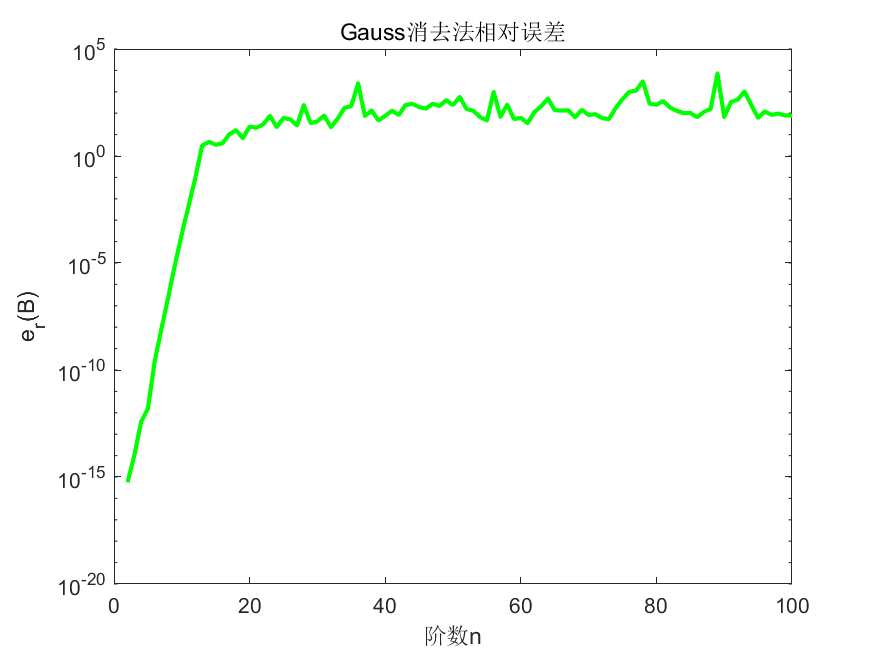
\includegraphics[width=0.8\textwidth]{../code/result/gausserror}
	\caption{\label{fig:4}Gauss消去法相对误差与阶数关系曲线图}
\end{figure}

\section{Jacobi矩阵迭代法}
设$H=D-L-U$,其中$D=diag(h_{11},h_{22},\cdots,h_{nn})$表示Hilbert矩阵$H$的对角线,$L$表示$H$的左下角元素的相反数,是一个下三角矩阵,$U$表示$H$的右上角元素的相反数,是一个上三角矩阵。因此,线性方程组$Hx=b$可以转换为$x=B_Jx+f$,其中$B_J=D^{-1}(L+U),f=D^{-1}b$,由此得到Jacobi迭代格式$x^{(k+1)}=B_Jx^{(k)}+f$。由于此种迭代格式只有当矩阵$B_J$的谱半径小于1时,迭代才是收敛的,因此,我们首先绘制出Jacobi迭代矩阵$B_J$的谱半径与阶数$n$的曲线图如图\ref{fig:5}所示,从图\subref{fig:b}中可以看出,当阶数$n>2$时,Jacobi迭代矩阵的谱半径就已经超过1了,因此当$n>2$时,Jacobi迭代法不收敛。当$n=2$时,我们设置当两次迭代的变化小于1e-6时,停止迭代,此时,Jicobi迭代相对误差为3.18555931744235e-07,误差比Gauss消去法在n=2时的误差还要大,因此,Jacobi迭代法不适合Hilbert矩阵线性方程组的求解。

\begin{figure}[!h] \centering 
	\subfigure[Jacobi迭代矩阵谱半径图] { \label{fig:a} 
		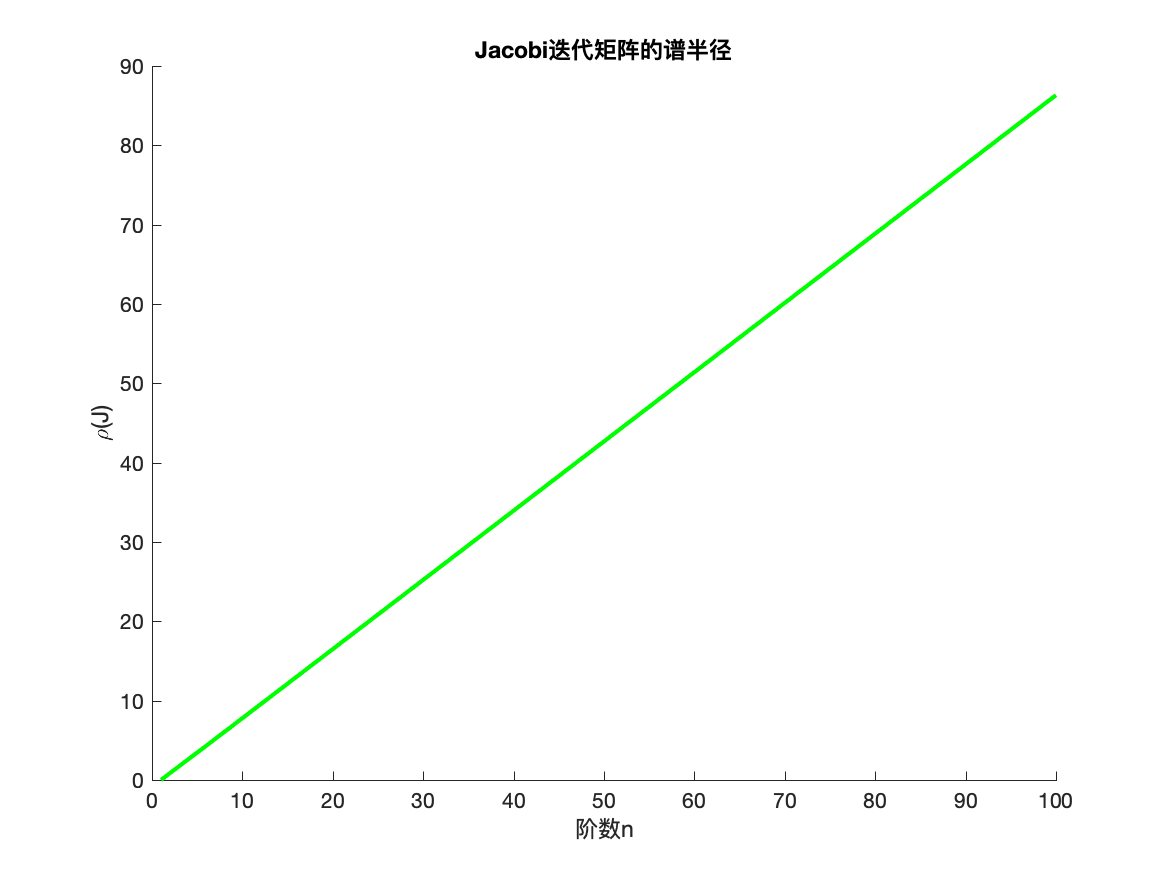
\includegraphics[width=0.48\columnwidth]{../code/result/jacobirho} 
	} 
	\subfigure[Jacobi迭代矩阵谱半径与1比较图] { \label{fig:b} 
		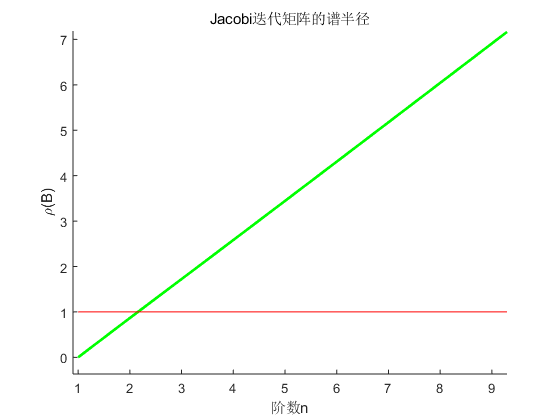
\includegraphics[width=0.48\columnwidth]{../code/result/jacobirho2} 
	} 
	\caption{Jacobi迭代矩阵谱半径图} 
	\label{fig:5} 
\end{figure}

\section{Gauss-Seidel矩阵迭代法}
设$H=D-L-U$,其中$D=diag(h_{11},h_{22},\cdots,h_{nn})$表示Hilbert矩阵$H$的对角线,$L$表示$H$的左下角元素的相反数,是一个下三角矩阵,$U$表示$H$的右上角元素的相反数,是一个上三角矩阵。因此,线性方程组$Hx=b$可以转换为$x=B_Gx+f$,其中$B_G=(D+L)^{-1}U,f=(D+L)^{-1}b$。与Jacobi矩阵迭代法类似,只有当矩阵$B_G$的谱半径小于1时,迭代才是收敛的,因此我们绘制出Gauss-Seidel迭代矩阵$B_G$的谱半径示意图如图\ref{fig:6}所示,从图中我们可以看出,当阶数$n\ge 13$时,谱半径已经近似$=1$了,因此此时Gauss-Seidel迭代法收敛速度很慢了。由此可知,Gauss-Seidel迭代法比Jacobi迭代法支持的Hilbert矩阵阶数高一点,但是仍然不能够用于高阶Hilbert矩阵线性方程组的求解。

\begin{figure}[!h]
	\centering
	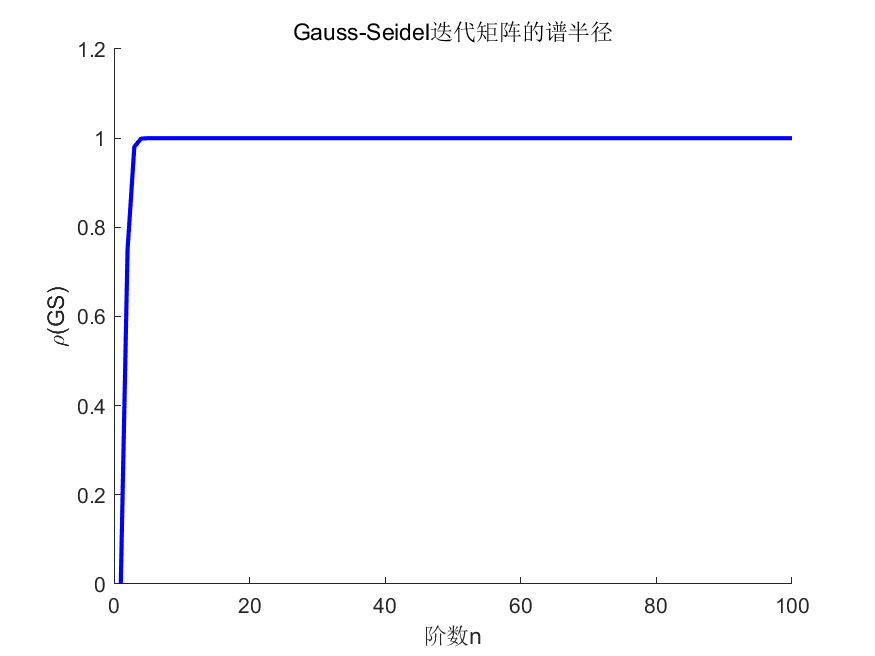
\includegraphics[width=0.8\textwidth]{../code/result/gsrho}
	\caption{\label{fig:6}Gauss-Seidel迭代矩阵谱半径与阶数n的关系图}
\end{figure}

\section{SOR迭代法}
设$H=D-L-U$,其中$D=diag(h_{11},h_{22},\cdots,h_{nn})$表示Hilbert矩阵$H$的对角线,$L$表示$H$的左下角元素的相反数,是一个下三角矩阵,$U$表示$H$的右上角元素的相反数,是一个上三角矩阵。因此,线性方程组$Hx=b$可以转换为$x=L_wx+f$,其中$L_w=(D-wL)^{-1}((1-w)D+wU),f=w*(D-wL)^{-1}b$。显然当$w=1$时,SOR迭代法即为Gauss-Seidel迭代法,并且根据上课学到的知识,只有当$0<w<2$时,SOR迭代法才收敛,对于不同的$w$,SOR迭代法的收敛速度也不同,因此我们首先寻找最优的$w$使得SOR迭代法的迭代矩阵$L_w$的谱半径最小,此时收敛速度最快。与GS迭代、Jacobi迭代类似,我们首先绘制出SOR迭代法的迭代矩阵$L_w$的谱半径如图\ref{fig:7}所示,从图中以及实验结果我们可以得到,当阶数$n>28$时,谱半径$\rho$接近1,因此此时SOR方法收敛很慢。由此可知,SOR迭代法比Jacobi迭代法以及Gauss-Seidel迭代法支持的Hilbert矩阵阶数更高一点,但是对于阶数过高的Hilbert矩阵求解,SOR迭代法仍然不可取。由于在图中不太容易直观的看出GS迭代法和SOR迭代法谱半径的不同,因此我们绘制出局部的图像进行对比,如图\ref{fig:8}所示,由此图可以看出,SOR迭代法的谱半径要比GS谱半径小,收敛速度较快。

\begin{figure}[!h]
	\centering
	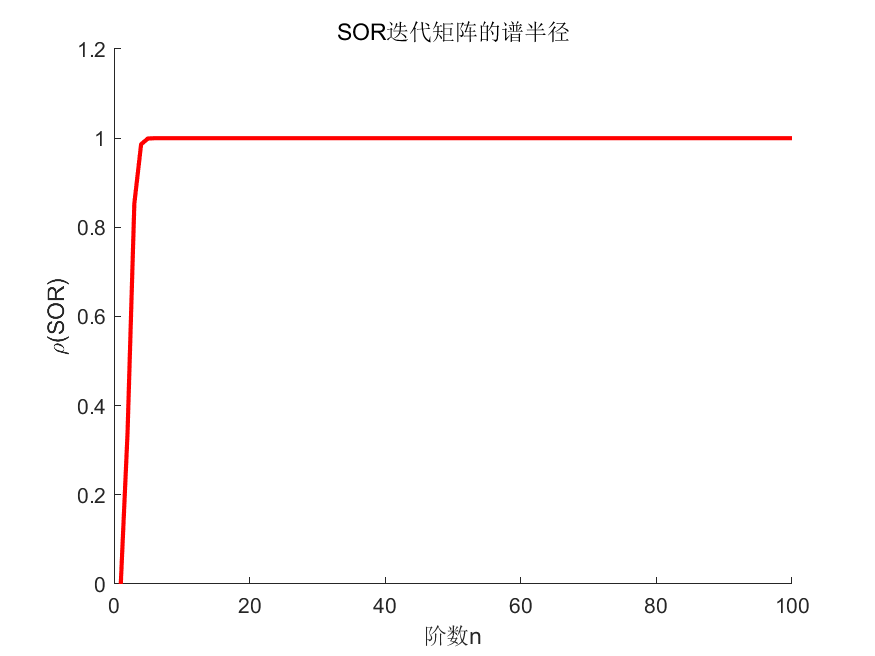
\includegraphics[width=0.8\textwidth]{../code/result/sorrho}
	\caption{\label{fig:7}SOR迭代矩阵谱半径与阶数n的关系图}
\end{figure}

\begin{figure}[!h] \centering 
	\subfigure[GS迭代矩阵谱半径局部图] { \label{fig:8a} 
		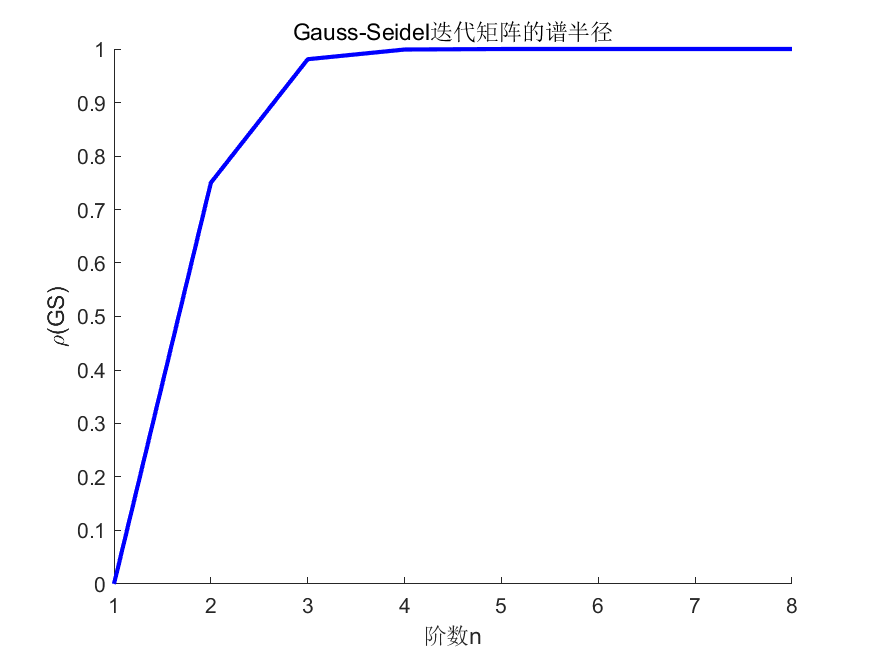
\includegraphics[width=0.48\columnwidth]{../code/result/gsrho2} 
	} 
	\subfigure[SOR迭代矩阵谱半径局部图] { \label{fig:8b} 
		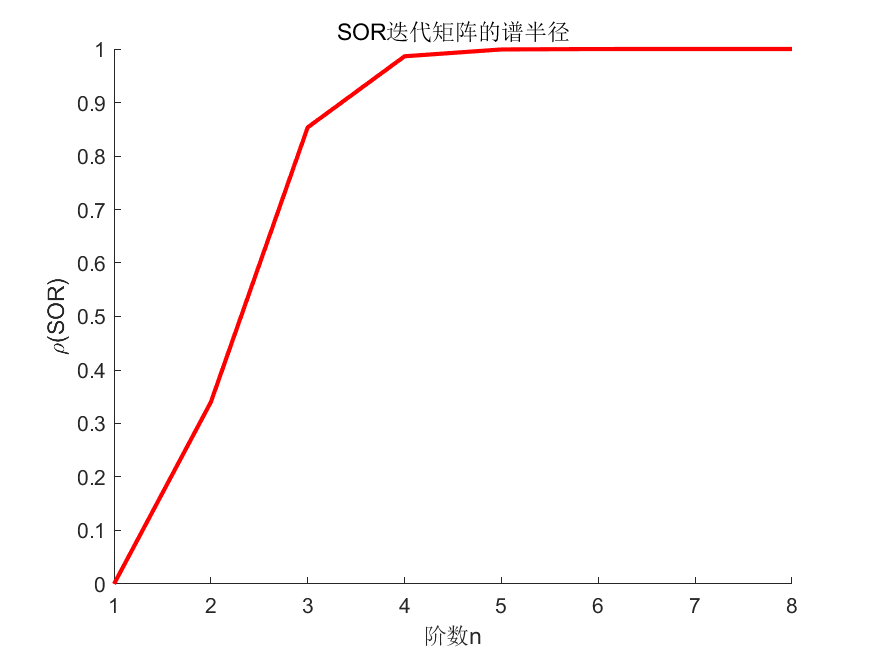
\includegraphics[width=0.48\columnwidth]{../code/result/sorrho2} 
	} 
	\caption{GS迭代矩阵和SOR迭代矩阵谱半径局部对比图} 
	\label{fig:8} 
\end{figure}

\section{实验结果对比}
在以上几节,我们讨论和分析了求解线性方程组的4种方法以及他们各自的性能,在此节我们将对其求出解得误差进行分析,我们设置阶数$n=2,5,10,20,50,100$,来计算相对误差,其中迭代法采用的初值均为0向量。

首先我们求出Jacobi迭代法经过100次迭代之后的相对误差如表\ref{tab:table3}所示,从中我们可以看出Jacobi迭代法对于n>2的Hilbert矩阵便已经不收敛了。

\begin{table}[htbp]
	\centering
	\caption{Jacobi迭代法相对误差与阶数关系表格}
	\label{tab:table3}
	\begin{tabular}{|c|c|c|c|}
		\hline
		阶数n & 谱半径$\rho(B_J)$& 迭代次数 &Jacobi迭代法的相对误差 \\
		\hline
		2 &0.866025403784439 &100 & 5.66321656347846e-07\\
		\hline
		5 &3.44414219116595 &100 & 6.18861899881230e+53\\
		\hline
		10 &7.77981513192998 &100 & 1.54832687372472e+89\\
		\hline
		20 &16.4920989837926 &100 & 6.66005666075554e+121\\
		\hline
		50 &42.6768950976645 &100 & 1.30642530458295e+163\\
		\hline
		100 &86.3374902073534 &100 & 5.21053762273348e+193\\
		\hline
	\end{tabular}
\end{table}

其次我们求出了GS迭代法的相对误差表,我们采用$\frac{||x^{(k)}-x^{(k-1)}s||_2}{||x^{(k-1)}||_2}<1e-6$来停止迭代,定义最大的迭代次数为20000,迭代结果如表\ref{tab:table4}所示。
	
	\begin{table}[htbp]
		\centering
		\caption{GS迭代法相对误差与阶数关系表格}
		\label{tab:table4}
		\begin{tabular}{|c|c|c|c|}
			\hline
			阶数n & 谱半径$\rho(B_{GS})$& 迭代次数 &GS迭代法的相对误差 \\
			\hline
			2 &0.750000000000000 &45 & 2.02811359558980e-06\\
			\hline
			5 &0.999957671222958 &7913 & 0.0138028658327348\\
			\hline
			10 &0.999999999997045 &17853 & 0.00873261631894775\\
			\hline
			20 &1.00000000000000 &20000 & 0.00873439429404305\\
			\hline
			50 &1.00000000000000 &20000 & 0.00959066207416708\\
			\hline
			100 &1.00000000000000 &20000 & 0.0101320928739749\\
			\hline
		\end{tabular}
	\end{table}

类似的,我们求出了SOR迭代法的误差表,我们依然采用$\frac{||x^{(k)}-x^{(k-1)}||_\infty}{||x^{(k-1)}||_\infty}<1e-6$来停止迭代,定义最大的迭代次数为20000,迭代结果如表\ref{tab:table5}所示。

\begin{table}[htbp]
	\centering
	\caption{SOR迭代法相对误差与阶数关系表格}
	\label{tab:table5}
	\begin{tabular}{|c|c|c|c|}
		\hline
		阶数n & 谱半径$\rho(B_{GS})$& 迭代次数 &GS迭代法的相对误差 \\
		\hline
		2 &0.340000000000000 &16 & 3.67239854881804e-08\\
		\hline
		5 &0.999190149180609 &9751 & 0.000542785068819967\\
		\hline
		10 &0.999999999871931 &12441 & 0.0381269338580335\\
		\hline
		20 &1.00000000000000 &5061 & 0.00712056341512206\\
		\hline
		50 &1.00000000000000 &15924 & 0.00553514159584128\\
		\hline
		100 &1.00000000000000 &9129 & 0.00599821418674224\\
		\hline
	\end{tabular}
\end{table}

从上述的结果中可以看出,Jacobi迭代法对于n>2的Hilbert矩阵是不收敛的,相对误差越来越大,不能用于此病态线性方程组的求解。GaussSeidel迭代法和SOR迭代法都是收敛的,相对误差并没有特别大。理论上,我们在SOR迭代法采用优化算法求出了最优松弛因子$w$,所以其收敛速度应该要比GS法的收敛速度快,但是从表\ref{tab:table4}和表\ref{tab:table5}中n=5时却出现了相反的情况,究其原因,应该是我们设置的收敛条件$\frac{||x^{(k)}-x^{(k-1)}||_\infty}{||x^{(k-1)}||_\infty}<1e-6$太严格导致会出现迭代次数盲目增加的情况。

由于我们知道正确解为$x^*=(1,1,\cdots,1)^T$,因此我们将收敛条件改为$\frac{||x^{(k)}-x^*||_2}{||x^{*}||_2}<1e-2$,将GS迭代法和SOR迭代法的结果列表如表\ref{tab:table6}所示,从这个表中我们便可以看出,SOR法的收敛速度确实要比GS法的收敛速度快。

\begin{table}[htbp]
	\centering
	\caption{SOR迭代法与GS迭代法收敛速度对比}
	\label{tab:table6}
	\begin{tabular}{|c|c|c|c|c|}
		\hline
		阶数n & GS法迭代次数& SOR法迭代次数 &GS迭代法的相对误差 & SOR法相对误差\\
		\hline
		2 & 16& 8& 0.00851756855749210& 0.00360255839563727\\
		\hline
		5 & 15527& 6688& 0.00999993017598135& 0.00999579098530880\\
		\hline
		10 & 15428& 9170& 0.00999959518767067& 0.00998574409924582\\
		\hline
		20 & 17301& 1829& 0.00999957638861157& 0.00999716337976600\\
		\hline
		50 & 16516& 3509& 0.00999978378907092& 0.00999838890291187\\
		\hline
		100 & 21622 & 4087& 0.00999998104858494& 0.00999876526546658\\
		\hline
	\end{tabular}
\end{table}

我们绘制出$n=10,50,100$时,迭代过程中相对误差的变化情况如图\ref{fig:9},\ref{fig:10},\ref{fig:11}所示,从图中我们可以清楚的看出SOR迭代法比GS法先到$10^{-2}$的误差,因此,SOR法收敛比GS法收敛快。

\begin{figure}[!h]
	\centering
	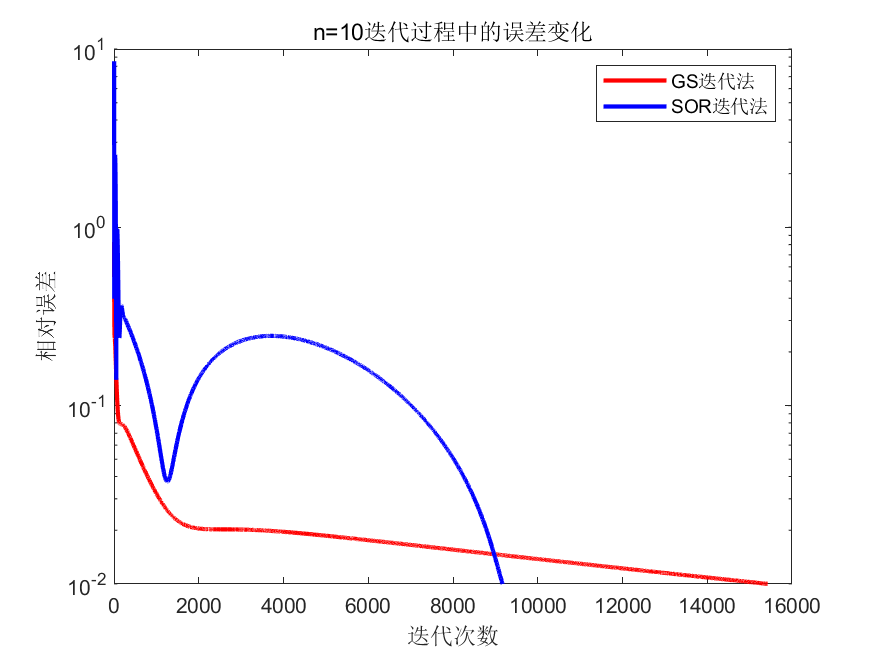
\includegraphics[width=0.8\textwidth]{../code/result/er10}
	\caption{\label{fig:9}n=10时迭代过程中相对误差的变化情况}
\end{figure}

\begin{figure}[!h]
	\centering
	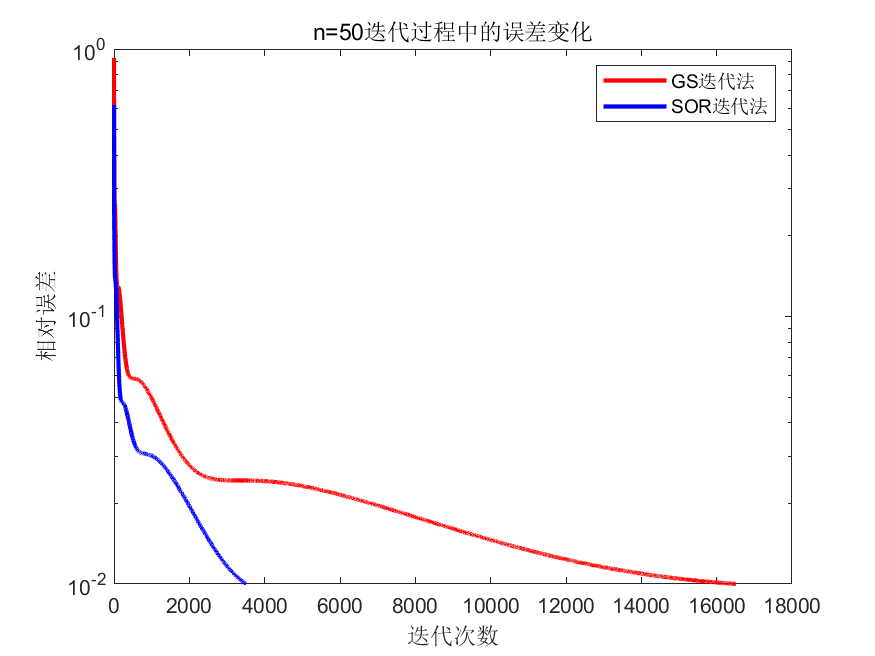
\includegraphics[width=0.8\textwidth]{../code/result/er50}
	\caption{\label{fig:10}n=50时迭代过程中相对误差的变化情况}
\end{figure}

\begin{figure}[!h]
	\centering
	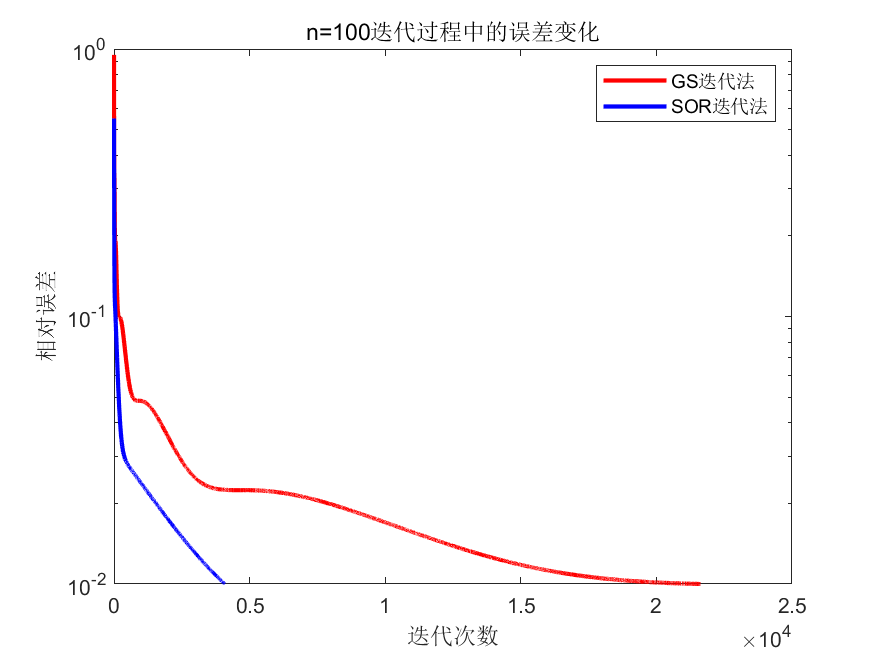
\includegraphics[width=0.8\textwidth]{../code/result/er100}
	\caption{\label{fig:11}n=100时迭代过程中相对误差的变化情况}
\end{figure}

此外,我们还绘制出了最优松弛因子关于阶数$n$的曲线如图\ref{fig:12}所示,从图中可以看出,阶数在13和14之间的突变是非常不合理的,考虑到我们在计算最优松弛因子时进行了$(D-wL)^{-1}$操作,由此可能引起极大的误差,因此在图\ref{fig:12}中只有当阶数n较小时的曲线才是正确的。

综上所述,对于Hilbert矩阵构成的病态线性方程组,Gauss消去法在阶数小于10时误差较小,可以求解,阶数较大时不能正确求解;Jacobi迭代法由于当阶数n>2时不收敛,因此不能用于求解;Gauss-Seidel迭代法和SOR迭代法可以用于求解此病态方程组,但是由于当阶数n较大时,收敛速度很慢,迭代次数很多,选取最优松弛因子的SOR迭代法比Gauss-Seidel迭代法收敛速度较快。

\begin{figure}[!h]
	\centering
	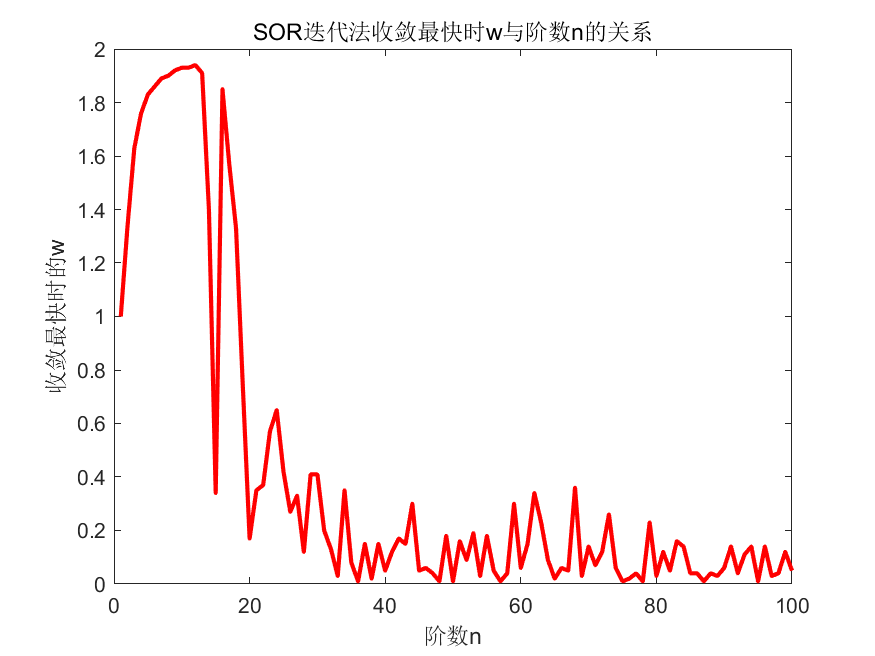
\includegraphics[width=0.8\textwidth]{../code/result/bestw}
	\caption{\label{fig:12}最优松弛因子与阶数n的关系图}
\end{figure}

\section{实验结论}
Hilbert 矩阵的 2-条件数随着阶数 n 的增大而呈指数增长,因此高阶
Hilbert 矩阵的病态性是毋庸置疑的,且阶数越高,解的误差应该越大,迭代法
收敛速度应该越慢。但是实验结果中常常在阶数 n 从 12 变为 13 时出现巨变,似
乎与理论不符合。事实上,无论是 Gauss 消去、Gauss-Seidel 迭代还是 SOR 迭
代,在阶数高时的求解步骤中就可能存在类似对病态矩阵求逆的操作,从而早成
高阶下的很多实验结果本身就有很大误差。而阶数 12 恰好又是这个临界点,因
此这种突变便可以理解了。寻找 Hilbert 矩阵 2-条件数和阶数 n 的关系时,一
开始直接用 cond 函数也发现在 n=12 出现了突变,但用专门的 invhilb 函数时便
能得到正确地结果,可见这种猜想是正确的。 
根据上述实验结果,发现对于 Hilbert 矩阵构成的病态线性方程组,Gauss
消去法无法准确求解。当矩阵的阶数不断增加时,解的相对误差也迅速增长。

用 Jacobi 迭代法求解 Hilbert 矩阵构成的病态线性方程,在阶数高于 2 时
便不再收敛。Jacobi 迭代矩阵的谱半径随阶数 n 的增大呈现近似线性增长,因
此 Jacobi 迭代法无法用于该病态方程组的求解。 

Gauss-Seidel 法和 SOR 法的迭代矩阵的谱半径在阶数 n 不断增长得过程中
趋近与 1,基于此不便于判断迭代法是否收敛。事实上,Hilbert矩阵是对称正定阵。令$[-1,1]$上的n次多项式$P(x)=a_0+a_1x+a_2x^2+\cdots+a_nx^n$,则式\ref{eq:1}。其中$H_n$为n阶Hilbert矩阵,因此可以看出$H_n$是对称正定的。由于我们有定理\ref{theorem1},所以Gauss-Seidel法和SOR法都是收敛的。但是由于在高阶(高于 5 阶)情况下,两者迭代矩阵的谱半
径都非常接近于 1,导致收敛速度很慢。前面的实验结果已经提到,要达到1e-2的相对误差,G-S 法要迭代上万次,SOR 法也要迭代几千次。至于阶数从 5、
10、20、50 、100变化过程中,收敛速度似乎波动稳定,原因也是矩阵本身的病态性导
致迭代法本身就是有较大误差的。事实上,收敛速度应该随着阶数增大而变慢。


\begin{equation}\label{eq:1}
\int_{-1}^{1}[P(x)]^2=[a_0,a_1,\cdots,a_2]H_n\left[
\begin{array}{c}
a_0 \\
a_1 \\
\vdots \\
a_n
\end{array}
\right]
\end{equation}

\begin{theorem}
	\label{theorem1}
	设$A\in \mathbb{R}^{n\times n}$是对称正定矩阵,且$0<w<2$,则SOR方法收敛。
\end{theorem}

综上所述,Jacobi 迭代法无法用于 Hilbert 矩阵构成的病态线性方程组的
求解;对于低阶(n=2~12)情况,可以用有预处理的 Gauss 消去法求解,此时解
的相对误差在可以接受的范围内,不采用迭代法的原因是收敛速度计算,慢复杂
度比高斯消去要高;对于高阶(n>12)的情况,只有采用迭代法才能保证精度,
但是收敛速度非常慢,迭代次数非常高,这也是病态线性方程组令人头疼的地方
所在吧。
\end{document}